\documentclass[border=5mm]{standalone}
\usepackage{pgfplots}
\usetikzlibrary{arrows.meta}
\pgfplotsset{compat=1.18}

\begin{document}
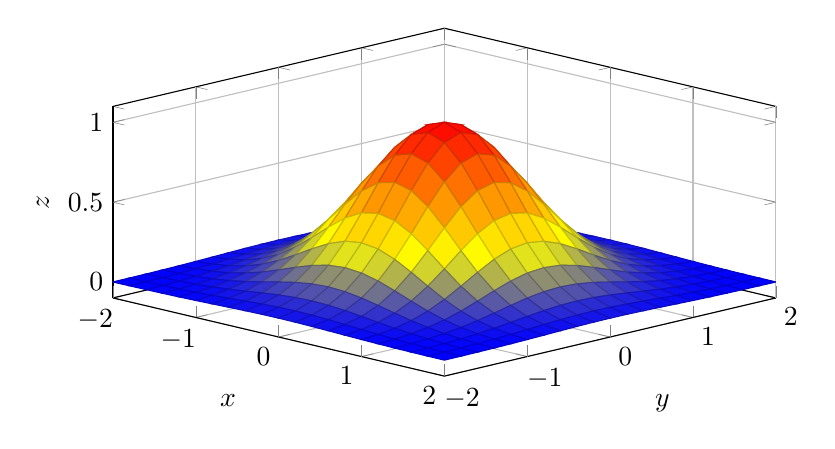
\begin{tikzpicture}[>=Stealth]
\begin{axis}[width=10cm,height=6cm,grid=major,view={45}{30},xlabel={$x$},ylabel={$y$},zlabel={$z$}]
\addplot3[surf,domain=-2:2,domain y=-2:2,samples=21]{exp(-x^2-y^2)};
\end{axis}
\end{tikzpicture}
\end{document}
